
%remark 

\begin{theorem}[Tunnel Troll Theorem]
Let $\Xi$ be a deterministic unary oritatami system of delay $\delta = 1$. 
At arity $\alpha \geq 3$, if $S[k] = t$ and $S[k+1] \neq \blacksquare$, then $\#bc(C_{k-1}) > \#bc(C_k)$.
On the other hand, at arity $\alpha = 2$, if there are indices $i,j$ such that $S[i..j+1]$ is either $bbt^{(j-i-1)}b$ or $bt^\ell bt^{j-i-1-\ell}b$ for some $\ell$, then $\#bc(C_{i-1}) > \#bc(C_j)$.
\end{theorem}

%%%%%%%%%%%%%%%%%%%%%%%%%%%%%%%%%%%%%%%%%%%%%%%%%%%%

\begin{lemma}
\label{TTT_entrance_Tab}
Let $\Xi$ be a deterministic unary oritatami system at delay $\delta = 1$, arity $\alpha =2$. 
Assume $\Xi$ stabilizes the transcript until $w[i-1]$. If $S[i+1] = b$ and $S[i+2] \in \{ t_s, t_o \} $, then $\#bc(C_{i-1}) > \#bc(C_{i})$.
\end{lemma}

\begin{proof}%[lemma \ref{TTT_entrance_Tab}]
See Fig.\ref{TTT_tunnel_direction}.
$S[i+2] \in \{ t_s, t_o \} $ means that $w[i+2]$ is stabilized by a tunnel section of type $S$ or $O$.
Thus,  its predecessor $w[i+1]$ must be inside the tunnel section, that is, $n_1$ and $n_2$ must be occupied.
Free bonds of $w[i]$, if any, cannot be used in future by another bead $w[j]$ because otherwise the part of transcript $w[i..j]$ and the bond between $w[i]$ and $w[j]$ would form a closed curve and the curve would cross the path of $C_{i-1}$ between $n_1$ and $n_2$, contradiction.
%Binding capabilities that $w[i]$ supplies are inactive according to Jordan curve theorem on $n_1$, $n_2$, and $w[i]$.
Therefore, if $w[i]$ forms a bond at its stabilization $\#bc(C_{i-1}) > \#bc(C_{i})$ holds.
We now prove that $w[i]$ must form a bond.


Suppose $w[i]$ ware stabilized without any bond, that is, by a tunnel.
For that the two points that are a neighbor of both $w[i-1]$ and $w[i]$ must be occupied already.
In addition, at least one of the neighbors of $w[i]$ must be free because $S[i+1] = b$.
Thus, only the case to be considered is Fig.~\ref{TTT_tunnel_direction} (middle) with $n_5$ being occupied (that is, $n_4$ is free).
In this case, before $w[i]$ is stabilized, at lest three neighbors of $n_2$ ware free and hence, a bead at $n_2$ was provided with one free bond and could form a bond with $w[i]$. \qed


\begin{figure}
  \begin{center}
    \begin{tabular}{ccc}
    
    
      \begin{minipage}{0.3\hsize}
      \centering
        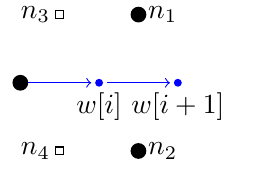
\begin{tikzpicture}
        \draw[->, white] (0:0)--(-120:1);
	 \draw[->,white] (120:0.8)--(120:0.1);%for adjustment
          
            \fill[blue] (0,0) circle [radius=0.05];
            \node[below] at (0,0) {$w[i]$};
            \node[below] at (0:1) {$w[i+1]$};

            \foreach \theta in {0}{
              \fill[transform canvas={shift=(\theta:1)},blue](0,0) circle [radius=0.05];
            }
            
            \foreach \theta in {60,-60,180}{
              \fill[transform canvas={shift=(\theta:1)}](0,0) circle [radius=0.1];
            }

            \foreach \theta in {120,-120}{
              \draw[transform canvas={shift=(\theta:1)}](-0.05,-0.05) rectangle (0.05,0.05);
            }
            
            \draw[->, blue] (180:0.9)--(180:0.1);
            \draw[->, blue] (0:0.1)--(0:0.9);

            \node[transform canvas={shift=(60:1)},right] {$n_1$};
            \node[transform canvas={shift=(-60:1)},right] {$n_2$};
            \node[transform canvas={shift=(120:1)},left] {$n_3$};
            \node[transform canvas={shift=(-120:1)},left] {$n_4$};


         % \node at (0,-2) {$t_{0}$};
        \end{tikzpicture}
      \end{minipage}

      

      \begin{minipage}{0.3\hsize}
      \centering
        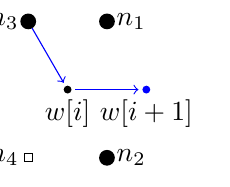
\begin{tikzpicture}
	\draw[->, white] (0:0)--(-120:1);
            \fill(0,0) circle [radius=0.05];
            \node[below] at (0,0) {$w[i]$};
            \node[below] at (0:1) {$w[i+1]$};

            \foreach \theta in {0}{
              \fill[transform canvas={shift=(\theta:1)},blue](0,0) circle [radius=0.05];
            }
            
            \foreach \theta in {60,-60,120}{
              \fill[transform canvas={shift=(\theta:1)}](0,0) circle [radius=0.1];
            }

            \foreach \theta in {180,-120}{
              \draw[transform canvas={shift=(\theta:1)}](-0.05,-0.05) rectangle (0.05,0.05);
            }
            
            \draw[->, blue] (120:0.9)--(120:0.1);
            \draw[->, blue] (0:0.1)--(0:0.9);

            \node[transform canvas={shift=(60:1)},right] {$n_1$};
            \node[transform canvas={shift=(-60:1)},right] {$n_2$};
            \node[transform canvas={shift=(120:1)},left] {$n_3$};
            \node[transform canvas={shift=(-120:1)},left] {$n_4$};
            \node[transform canvas={shift=(180:1)},left] {$n_5$};

          %\node at (0,-2) {$t_{\pm 60}$};
        \end{tikzpicture}
      \end{minipage}

      \begin{minipage}{0.3\hsize}
      \centering
        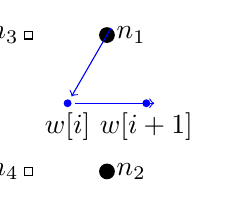
\begin{tikzpicture}
        \draw[->, white] (0:0)--(-120:1);
            \fill[blue](0,0) circle [radius=0.05];
            \node[below] at (0,0) {$w[i]$};
            \node[below] at (0:1) {$w[i+1]$};

            \foreach \theta in {0}{
              \fill[transform canvas={shift=(\theta:1)}, blue](0,0) circle [radius=0.05];
            }
            
            \foreach \theta in {60,-60}{
              \fill[transform canvas={shift=(\theta:1)}](0,0) circle [radius=0.1];
            }

            \foreach \theta in {180,-120,120}{
              \draw[transform canvas={shift=(\theta:1)}](-0.05,-0.05) rectangle (0.05,0.05);
            }
            
            \draw[->, blue] (60:1.1)--(60:0.1);
            \draw[->, blue] (0:0.1)--(0:1.1);

            %\node[transform canvas={shift=(0:1)},below] {$n_0$};
            \node[transform canvas={shift=(60:1)},right] {$n_1$};
            \node[transform canvas={shift=(-60:1)},right] {$n_2$};
            \node[transform canvas={shift=(120:1)},left] {$n_3$};
            \node[transform canvas={shift=(-120:1)},left] {$n_4$};
            \node[transform canvas={shift=(180:1)},left] {$n_5$};

         % \node at (0,-2) {$t_{\pm 120}$};
        \end{tikzpicture}
      \end{minipage}
      
    \end{tabular}
    \caption{Direction into a entrance}
    \label{TTT_tunnel_direction}
  \end{center}
\end{figure}

\end{proof}


%%%%%%%%%%%%%%%%%%%%%%%%%%%%%%%%%%%%%%%%%%%%%%%%%%%%

\begin{lemma}
\label{TTT_exit}
Let $\Xi$ be a deterministic unary oritatami system of delay $\delta = 1$ and arity $\alpha =2$.
%Let $w[i]$ be a bead which is stabilized at the exit of a tunnel.
If $S[h..i+1] = bt^{(i-h)}b$ for some $h<i-1$, then $\#bc(C_{i-2}) \geq \#bc(C_i)$, and hence, $\#bc(C_{h-1}) \geq \#bc(C_i)$.
If $h < i-1$, then the second inequality is strengthened as $\#bc(C_{h-1}) > \#bc(C_{i})$.
%if we assume $\#bc(C_{i-2}) - \#bc(C_{i-1}) = a$, then $\#bc(C_{i}) - \#bc(C_{i-1}) \leq a$.
\end{lemma}

\begin{proof}%[Lemma~ \ref{TTT_exit}]
Since the binding capability never increases inside a tunnel, we just need to consider the exit of a tunnel.
See Fig.\ref{TTT_tunnel_exit}. 
At least one of points $n_1$ or $n_2$ must be free because otherwise $w[i]$ would be inside of a tunnel, that is, $S[i+1]$ would not be $b$.

%If $i - h > 1$ and $j$ is such that $h \leq j<i$, then $\#bc(C_{j-1}) \geq \#bc(C_{j})$ because all neighbors of $w[j]$ are occupied by beads forming the tunnel so that any $w[i+1..]$ cannot reach neighbors of $w[j]$. 
%Thus, inside this tunnel, binding capabilities never increased.


Let $a$ be the number of bonds $w[i-1]$ forms, that is, $\#bc(C_{i-2}) - \#bc(C_{i-1}) = a$. Then, $\#bc(C_{i}) - \#bc(C_{i-1}) \leq a$ as follows.

\begin{itemize}
\item{Case of both $n_1$ and $n_2$ being free}\\
  This case can be regarded the same as entrance. See Fig.\ref{TTT_tunnel_exit} (Left). Predecessor $n_5$ has to be bound to $n_4$ and $n_5$ because both of $n_3$ and $n_4$ have binding capabilities. Hence, $a \geq 2$. This time, $\alpha = 2$, that is, this case $\#bc(C_{i}) - \#bc(C_{i-1}) \leq a$.
  
\item{Case of $n_1$ is occupied}\\
  See Fig.\ref{TTT_tunnel_exit} (Right). If $n_1$ is occupied, then $n_2$ is free so that $n_5$ has to be bound $n_4$. Hence,  $a \geq 1$. This case can supply two binding capabilities but $p^\prime$ can bind to only one of $n_0$ or $n_2$ because $n_0$ or $n_2$ will be occupied by the successor of $p^\prime$. Therefore, this case $\#bc(C_{i}) - \#bc(C_{i-1}) \leq a$.
  
\end{itemize}

Thus,$\#bc(C_{i-2}) \geq \#bc(C_i)$ , and hence, $\#bc(C_{h-1}) \geq \#bc(C_i)$.
If $h < i-1$, then the second inequality is strengthened as $\#bc(C_{h-1}) > \#bc(C_{i})$ because $S[h] = b$, that is, $\#bc(C_{h-1}) > \#bc(C_h)$ and $\#bc(C_{h}) \geq \#bc(C_i)$. \qed

\begin{figure}
  \centering
    \begin{tabular}{cc}
    \centering
      \begin{minipage}{0.45\linewidth}
      \centering
        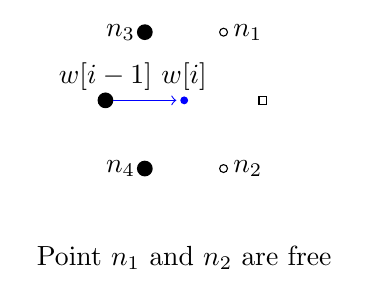
\begin{tikzpicture}
	\draw[white] (0:0) -- (120:1);
	\draw[white] (0:0) -- (-60:1);
	\draw[white] (0:0) -- (0:1);

            \fill[blue](0,0) circle [radius=0.05];
            \node[above] at (0,0) {$w[i]$};

            
            \foreach \theta in {120,-120,180}{
              \fill[transform canvas={shift=(\theta:1)}](0,0) circle [radius=0.1];
            }

            \foreach \theta in {0}{
              \draw[transform canvas={shift=(\theta:1)}](-0.05,-0.05) rectangle (0.05,0.05);
            }
            \draw (-60:1) circle [radius=0.05];
            \draw (60:1) circle [radius=0.05];

            \draw[->, blue] (180:0.9)--(180:0.1);



            \node[transform canvas={shift=(60:1)},right] {$n_1$};
            \node[transform canvas={shift=(-60:1)},right] {$n_2$};
            \node[transform canvas={shift=(120:1)},left] {$n_3$};
            \node[transform canvas={shift=(-120:1)},left] {$n_4$};
            \node[transform canvas={shift=(180:1)},above] {$w[i-1]$};

          \node at (0,-2) {Point $n_1$ and $n_2$ are free};
        \end{tikzpicture}
      \end{minipage}

      \begin{minipage}{0.45\linewidth}
      \centering
        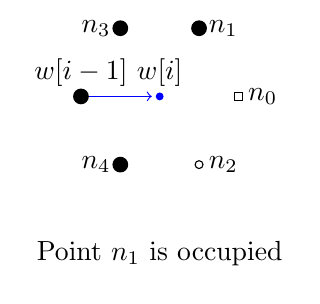
\begin{tikzpicture}
	\draw[white] (0:0) -- (0:1);
	\draw[white] (0:0) -- (120:1);
	\draw[white] (0:0) -- (-90:2);

            \fill[blue](0,0) circle [radius=0.05];
            \node[above] at (0,0) {$w[i]$};
            
            \foreach \theta in {120,-120,180,60}{
              \fill[transform canvas={shift=(\theta:1)}](0,0) circle [radius=0.1];
            }

            \foreach \theta in {0}{
              \draw[transform canvas={shift=(\theta:1)}](-0.05,-0.05) rectangle (0.05,0.05);
            }
            \draw (-60:1) circle [radius=0.05];

            \draw[->, blue] (180:0.9)--(180:0.1);

            \node[transform canvas={shift=(0:1)},right] {$n_0$};
            \node[transform canvas={shift=(60:1)},right] {$n_1$};
            \node[transform canvas={shift=(-60:1)},right] {$n_2$};
            \node[transform canvas={shift=(120:1)},left] {$n_3$};
            \node[transform canvas={shift=(-120:1)},left] {$n_4$};
            \node[transform canvas={shift=(180:1)},above] {$w[i-1]$};


          
          \node at (0,-2) {Point $n_1$ is occupied};
        \end{tikzpicture}
      \end{minipage}
    \end{tabular}
    \caption{Exit of Tunnel}
    \label{TTT_tunnel_exit}
\end{figure}
\end{proof}

%%%%%%%%%%%%%%%%%%%%%%%%%%%%%%%%%%%%%%%%%%%%%%%%%%%%



\begin{lemma}
\label{TTT_tunnelC_lemma}
Let $\Xi$ be a deterministic unary oritatami system of delay $\delta = 1$, arity $\alpha = 2$. If there are indices $i,j$ such that $S[i..j+1]$ is either $bbt^{(j-i-1)}b$ and $S[i+2] = t_a$ or $bt^\ell bt^{j-i-1-\ell}b$ for some $\ell$ and $S[i+l+2] = t_a$, then $\#bc(C_{i-1}) > \#bc(C_j)$.
\end{lemma}

%\begin{lemma}
%\label{TTT_tunnelC_lemma}
%Let $\Xi$ be a deterministic unary oritatami system of delay $\delta = 1$, arity $\alpha = 2$. We assume $S[h..i+1] = bt^{(i-h)}b \quad (1<h<i)$. If at least one of $w[h+1..i]$ is stabilized by tunnel $C$, then $\#bc(C_{h-3}) > \#bc(C_{h+1})$ and $\#bc(C_{h-3}) > \#bc(C_i)$.
%\end{lemma}


\begin{proof}[Lemma~ \ref{TTT_tunnelC_lemma}]
Let $\Xi$ be a unary oritatami system at $\delta = 1, \alpha = 2$.
Assume $S[h..i+1] = bt^{i-h}b (h<i)$. If at least one of $w[h+1..i]$ are stabilized by tunnel $C$, then only $w[h+1]$ can use tunnel $C$ because if $w[g]$ which is one of $w[h+2..i]$, with $h+2 \leq g \leq i$ is stabilized by tunnel $C$, $C_g$ is a terminal.


Let us consider stabilization $S[h-1..h+1] = tbt$ or $S[h-1..h+1] = bbt$ as follows. In result, $\#bc(C_{h-3}) > \#bc(C_{h+1})$. In addition according to Lemma~\ref{TTT_exit} $\#bc(C_{h+1}) \geq \#bc(C_{i})$. Thus, $\#bc(C_{h-3}) > \#bc(C_{h+1})$ and $\#bc(C_{h-3}) > \#bc(C_{i})$.
\\

\subsubsection{Case of $S[h-1..h+1] = bbt$}
See Fig.~\ref{TTT_tunnelC_enter_usingBond}.
If $w[h-1]$ forms one bond, then it leaves one free bond, but it is consumed by $w[h+1]$.
In addition, $w[h]$ has to bound.
Thus, in this cases, binding capability decreases by 1.
If $w[h-1]$ forms two bonds, then it does not leave any bond.
In addition, $w[h]$ has to be bound.
Thus, in this case, even if $w[h+1]$ supplies two free bonds, binding capability decreases by 1.




\begin{figure}
  \begin{center}
        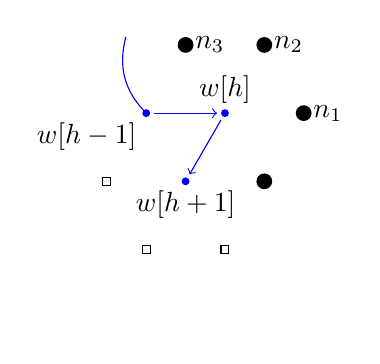
\begin{tikzpicture}
        \draw[->,white] (-70:0.1) -- (-70:3);
          \foreach \theta in {60,-60,120,0}{
            \fill[transform canvas={shift=(\theta:1)}](0,0) circle [radius=0.1];
          }

          \fill[blue](180:1) circle [radius=0.05];
          \fill[blue](0:0) circle [radius=0.05];

          \draw[transform canvas={shift=(180:1)}, blue] (105:1) edge[bend right] (105:0);
          \draw[->, blue] (180:0.9) -- (180:0.1);
          \draw[->, blue] (-120:0.1) -- (-120:0.9);

          \node[below left] at (180:1) {$w[h-1]$};
          \node[above] at (0:0) {$w[h]$};
          \node[below] at (-120:1) {$w[h+1]$};

          \node[right] at (120:1) {$n_3$};
          \node[right] at (60:1) {$n_2$};
          \node[right] at (0:1) {$n_1$};

          \begin{scope}[shift=(-120:1)]
            \fill[blue](0,0) circle [radius=0.05];
            \foreach \theta in {-120,-60,180}{
              \draw[transform canvas={shift=(\theta:1)}](-0.05,-0.05) rectangle (0.05,0.05);
            }
            
          \end{scope}
        \end{tikzpicture}
    \caption{Case of $S[h-1..h+1] = bbt$}
    \label{TTT_tunnelC_enter_usingBond}
  \end{center}
\end{figure}


\subsubsection{Case of $S[h-1..h+1] = tbt$}
Fig.\ref{TTT_tunnelC_enter_usingTunnel} exhibits all the two kinds of stabilization depending on structures of tunnel C.

\begin{itemize}
\item{Left of Fig.\ref{TTT_tunnelC_enter_usingTunnel}}\\
  In this figure, Bead $n_4$ has at least one binding so that $w[h-1]$ has to bound $n_4$. Moreover, $w[h]$ has to bind to one of $n_1, n_2, n_3$ in order to stabilize deterministically. On the other hand, $w[h+1]$ can supply two bindings but has only two free neighbors. One of them is occupied by a successor. Therefore $w[h+1]$ can only bind one of $n_5, n_6$, that is, $w[h+1]$ supplies at most one binding. Thus, this case $\#bc(C_{h-1}) > \#bc(C_{h+1})$.

\item{Right of Fig.\ref{TTT_tunnelC_enter_usingTunnel}}\\
  These cases are divided on number of capabilities that $w[h-1]$ consumes.
  \begin{itemize}
  \item[-]{$w[h-1]$ does not consume any bindings}\\
  According to Lemma~\ref{TTT_exit}, $\#bc(C_{h-3}) \geq \#bc(C_{h-1})$ because of $S[h-1] = t$.
    $w[h]$ has to bound one of $n_1, n_2, n_3$ in order to stabilize deterministically so that  $\#bc(C_{h-1}) > \#bc(C_{h})$.
    $w[h+1]$ has to be bound to $w[h-1]$ because $w[h-1]$ has bindings, that is, $w[h+1]$ consumes at least one hand and supplies at most one hand so that $\#bc(C_{h}) \geq \#bc(C_{h+1})$. Thus, in this cases $\#bc(C_{h-3}) > \#bc(C_{h+1})$.
%     This time, let us consider either $n_4$ is occupied or not. If $n_4$ is occupied, then $w[h-1]$ has no active bindings that is this situation consumes some binding capabilities. If $n_4$ is free and $w[h+2]$ is stabilized in $n_4$, then $w[h-1]$ has to bind $w[h+2]$. Therefore, In this case, stabilization of $w[h-1..h+2]$ consumes some bindings. If $n_4$ is free and $w[h+2]$ is stabilized except $n_4$, then this oritatami system has to use two binding capabilities in order to bind $w[h+2]$. Therefore, in this case consumes some bindings. Thus in this cases $\#bc(C_{h-1}) > \#bc(C_{h+2})$.

  \item[-]{$w[h-1]$ consumes one binding}\\
    In this case, $w_{h}$ has to be bound one of $n_1, n_2, n_3$. In addition, $w[h-1]$ and $w[h+1]$ are not supply any bindings. Thus, in this cases consume some binding capabilities.
  \item[-]{$w[h-1]$ consumes two bindings}\\
    In this case, $w[h-1]$ already consumes two binding. $w[h]$ has to be bound. $w[h+1]$ supplies two bindings. Thus, in this cases $\#bc(C_{h-1}) > \#bc(C_{h+1})$.
   
  \end{itemize}
\end{itemize}
\begin{figure}
  \centering
    \begin{tabular}{cc}
      
      \begin{minipage}{0.48\hsize}
      \centering
        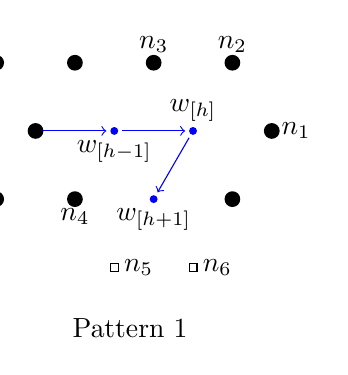
\begin{tikzpicture}

          \fill[transform canvas={shift=(0:0)}](0,0) circle [radius=0.1];
          
          \foreach \theta in {60,-60,120,-120,180}{
            \fill[transform canvas={shift=(\theta:1)}](0,0) circle [radius=0.1];
          }

          \fill[blue](0:1) circle [radius=0.05];
          \draw[->, blue] (0:0.1)--(0:0.9);

          \node[below] at (-60:1) {$n_4$};

          \begin{scope}[shift=(0:2)]
            \fill[blue](0,0) circle [radius=0.05];

            
            \foreach \theta in {120,60,-60,0}{
             \fill[transform canvas={shift=(\theta:1)}](0,0) circle [radius=0.1];
            }

            \draw[->, blue] (180:0.9)--(180:0.1);
            \draw[->, blue] (-120:0.1)--(-120:0.9);

            \node[below] at (180:1) {$w_{[h-1]}$};
            \node[above] at (0:0) {$w_{[h]}$};
            \node[below] at (-120:1) {$w_{[h+1]}$};

            \node[above] at (120:1) {$n_3$};
            \node[above] at (60:1) {$n_2$};
            \node[right] at (0:1) {$n_1$};

            \begin{scope}[shift=(-120:1)]
              \fill[blue](0,0) circle [radius=0.05];
              \foreach \theta in {-120,-60}{
                \draw[transform canvas={shift=(\theta:1)}](-0.05,-0.05) rectangle (0.05,0.05);
              }

              \node[right] at (-120:1) {$n_5$};
              \node[right] at (-60:1) {$n_6$};
            \end{scope}
            
          \end{scope}

          \node at (1.2,-2.5) {Pattern 1};
        \end{tikzpicture}
      \end{minipage}

      \begin{minipage}{0.48\hsize}
      \centering
        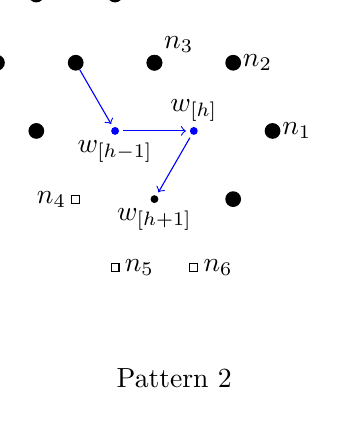
\begin{tikzpicture}

          \fill(0,0) circle [radius=0.1];
          
          \foreach \theta in {60,0,120,-120,180}{
            \fill[transform canvas={shift=(\theta:1)}](0,0) circle [radius=0.1];
          }

          \draw[->, blue] (-60:0.1)--(-60:0.9);


          \begin{scope}[shift=(-60:1),shift=(0:1)]
            \fill[blue](0,0) circle [radius=0.05];
            \fill[blue](180:1) circle [radius=0.05];

            
            \foreach \theta in {120,60,0,-60}{
              \fill[transform canvas={shift=(\theta:1)}](0,0) circle [radius=0.1];
            }

            \draw[->, blue] (180:0.9)--(180:0.1);
            \draw[->, blue] (-120:0.1)--(-120:0.9);

            \node[below] at (180:1) {$w_{[h-1]}$};
            \node[above] at (0:0) {$w_{[h]}$};
            \node[below] at (-120:1) {$w_{[h+1]}$};

            \node[above right] at (120:1) {$n_3$};
            \node[right] at (60:1) {$n_2$};
            \node[right] at (0:1) {$n_1$};

            \begin{scope}[shift=(-120:1)]
              \fill(0,0) circle [radius=0.05];
              \foreach \theta in {180,-120,-60}{
                \draw[transform canvas={shift=(\theta:1)}](-0.05,-0.05) rectangle (0.05,0.05);
              }

              \node[left] at (180:1) {$n_4$};
              \node[right] at (-120:1) {$n_5$};
              \node[right] at (-60:1) {$n_6$};
            \end{scope}
            
          \end{scope}

          \node at (1.25,-4) {Pattern 2};
        \end{tikzpicture}
      \end{minipage}

      
      
    \end{tabular}
    \caption{Case of $S[h-1..h+1] = tbt$}
    \label{TTT_tunnelC_enter_usingTunnel}
\end{figure}



\end{proof}



%%%%%%%%%%%%%%%%%%%%%%%%%%%%%%%%%%%%%%%%%%%%%%%%%%%%
%%
%%%%
%%%%%%
%%%%%%%%
%%%%%%%%%%%%%%%%%%%%%%%%%%%%%%%%%%%%%%%%%%%%%%%%%%%%

\proof%{Proof of Tunnel Troll Theorem}
Each bead in the transcript is bound either inside a tunnel or outside. If a bead is stabilized inside a tunnel, 
then it has at most one free neighbor, and hence its successor it to be stabilized there.
Moreover, if a bead is stabilized outside a tunnel, then its position is either an entrance of a tunnel or not.

Tunnel sections have three possible shapes up to symmetry : straight($S$), obtuse($O$) and acute($A$) turn (Fig. \ref{TTT_tunnel}), and we will consider each of those. 

%\begin{lemma}
%\label{TTT_neighbor_lemma}
%For unary transcripts at $\delta = 1$, if a bead has no free hand, then at least $\alpha + 2$ of its neighbors have to be occpied.
%\end{lemma}

Let us first consider cases of $\delta \geq 3, \alpha = 1$. 
See Fig.~\ref{TTT_tunnel_exit}. Consider the stabilization of $w[i]$. 
This bead $w[i]$, once stabilized, shares two neighbors with its predecessor $w[i-1]$, which are denoted by $n_3, n_4$. 
Both of them have been already occupied because $S[i] = t$. 

Since $S[i+1] \neq \blacksquare$, at least one of the other three neighbors, denoted by $n_0, n_1, n_2$, must be free. 
Assume that in the neighborhood of $w[i]$, there are two beads with one free neighbor even after $w[i]$ is stabilized. 
Before the stabilization of $w[i]$, such a bead had two free neighbors, and hence, is provided with at least one free bond. 
Thus, $w[i]$ is to be bonded to these two beads, and it decreases the binding capability by at least 1. 
It now suffices to check that this assumption holds no matter how $n_0, n_1, n_2$ are occupied as long as at least one of them is left free. 

Next, we consider the case of $\delta = 2, \alpha = 1$. We assume there is an index $h$ such that $S[h-1..h+1] = bbt$ or $S[h-1..h+1] = tbt$. According to Lemma~\ref{TTT_entrance_Tab}, if $w[h+1]$ is stabilized by tunnel $A$ or $B$, then $\#bc(C_{h-1}) > \#bc(C_{h})$. Also,  According to Lemma~\ref{TTT_tunnelC_lemma}, if $w[h+1]$ is stabilized by tunnel $C$, then $\#bc(C_{h-3}) > \#bc(C_{h+1})$.
On the other hand, if $S[k..l] = bt^{l-k}b$, then $\#bc(C_{k-1}) \geq \#bc(C_{l})$ because of Lemma~\ref{TTT_exit}. Therefore, if there are indices $i$ and $j$ such that $S[i..j+1] = bbt^{(j-i-1)}b$ or $S[i..j+1] = bt^mbt^nb \quad (m + n = j-i-1)$, then $\#bc(C_{i-1}) > \#bc(C_{j})$.

\qed






%%%%%%%%%%%%%%%%%%%%%%%%%%%%%%%%%%%%%%%%%%%%%%%%%%%%%%%%%
%/////////////////////////////////////////////////
%%%%%%%%%%%%%%%%%%%%%%%%%%%%%%%%%%%%%%%%%%%%%%%%%%%%%%%%%


\subsection{On structures provided by a unary and $\delta = 1$ oritatami system}
\begin{theorem}[$\delta= 1, \alpha=2$]
Let $\Xi$ be a unary oritatami system of $\delta = 1, \alpha = 2$. It can yield infinite structures but they are only zig-zag conformation.
\end{theorem}

\begin{proof}
By Tunnel Troll Theorem, any tunnel sections which represented in $bbt^+$ or $bt^+bt^+$ consume binding capabilities. If the sequence $S$ is free from any subsequence of the form $bt^+bt^+$, then it can factorize as $S = u_1 u_2 u_3 \cdots$ for some $u_1 , u_2 , u_3 , \cdots \in \{b\} \cup bbt^+$. Assume the length of $\sigma$ is $n$, seed supplies at most $2n$ binding capabilities. Therefore formula \ref{TTT_only_bond} hold.

\begin{eqnarray}
  \exists i \in \mathbb{N} \quad s.t. \quad u_{i-1} , u_i , u_{i+1} , u_{i+2} , \cdots \in \{ b \}
  \label{TTT_only_bond}
\end{eqnarray}


Let us represent $S$ as $S[i.i+1...] = v_i v_{i+1} v_{i+2} \cdots$ for some $v_i, v_{i+1}, v_{i+2}, \cdots \in \{ a, o\}$ where if $v_k$ is $a$, then $v_{k+1}$ is bound to $v_{k-1}$, if $v_k$ is $o$, then $v_{k+1}$ is NOT bound to $v_{k-1}$.


Let us consider the case of $v_k$ is $o$. See Fig.\ref{TTT_case_of_o}. $w[i-1]$ consumes some binding capabilities because $v_{i-1}$ is $b$. If the number of $w[i-1]$'s bindings is one binding, then $w[i+1]$ has to be bound except $n_1$ or $n_2$ so that $w[i+1]$ must consumes two bindings except the case of $n_1$ and $n_2$ are occupied and $w[i]$ consumes at least one binding. If $n_1$ and $n_2$ are occupied, then $w[i-1]$'s bindings are inactive, that is, $w[i-1]$ consumes two binding capabilities. Therefore, this case consumes binding capabilities. If $w[i-1]$ dose Not have any bindings, then $w[i-1]$ already consumes two bindings. In addition, $w[i]$ and $w[i+1]$ consume at least one binding. Therefore this case consumes binding capabilities. Thus, the formula \ref{TTT_only_a} hold and according to the formula \ref{TTT_only_bond} and the formula \ref{TTT_only_a}, the formula \ref{TTT_structure} is hold. Thus, in this case, oritatami system can yield infinite structures but they are only zig-zag conformation.

\end{proof}

\begin{eqnarray}
  \exists j \in \mathbb{N} \quad s.t. \quad u_j , u_{j+1} , u_{j+2} , \cdots \in \{ a \}
  \label{TTT_only_a}
\end{eqnarray}

\begin{eqnarray}
  | S | > \forall m \in \mathbb{N} \quad \to \quad \exists n \in \mathbb{N} \quad s.t. \quad S[n], S[n+1], \cdots \in \{ a \}
  \label{TTT_structure}
\end{eqnarray}

\begin{figure}
  \begin{center}
    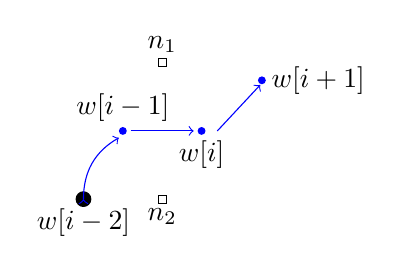
\begin{tikzpicture}
      
      \fill[transform canvas={shift=(-120:1)}](0,0) circle [radius=0.1];
      
      \fill[blue](0:0) circle [radius=0.05];
      \fill[blue](0:1) circle [radius=0.05];
      \fill[shift=(0:1), blue](40:1) circle [radius=0.05];

      \draw[->, blue] (-120:1) edge[bend left] (-120:0.1);
      \draw[->, blue] (0:0.1) -- (0:0.9);
      \draw[->,transform canvas={shift=(0:1.2)}, blue] (50:0) -- (47:0.8);
      
      \draw[shift=(60:1)](-0.05,-0.05) rectangle (0.05,0.05);
      \draw[shift=(-60:1)](-0.05,-0.05) rectangle (0.05,0.05);
      
      \node[below] at (-120:1) {$w[i-2]$};
      \node[above] at (0:0) {$w[i-1]$};
      \node[below] at (0:1) {$w[i]$};
      \node[right, shift=(0:1)] at (40:1) {$w[i+1]$};

      \node[above] at (60:1) {$n_1$};
      \node[below] at (-60:1) {$n_2$};
        
    \end{tikzpicture}
    \caption{Case of $S[i]$}
    \label{TTT_case_of_o}
  \end{center}
\end{figure}

\begin{theorem}[$\delta = 1, \alpha = 3$]
Let $\Xi$ be a unary oritatami system of $\delta = 1, \alpha = 3$. It can yield only finite structures whose size is $O(n)$.
\end{theorem}

\begin{lemma}
\label{TTT_a3_2b_lemma}
 Let $p$ be a point whose neighbors is occupied at least two point. If $w[i]$ is not stabilized and $w[i-1]$ includes neighbors of $p$, then $w[i]$ is stabilized at $p$ with at least one bond, $w[i]$ is stabilized at another point of $p$ otherwise with at least two bond except any neighbors of $p$ is occupied.
\end{lemma}

\begin{proof}[proof of lemma]
Assume the transcript is stabilized until $w[i-1]$. One of neighbors of $p$ is not $w[i-1]$ where this bead regards $n_1$. If $w[i-1]$ include neighbors of $p$ and $w[i]$ is stabilized at another point of $p$ with one bond. Then, any neighbors do not have bond without $w[i-1]$. Neighbors of $n_1$ have to be occupied at least five according to lemma \ref{TTT_neighbor_lemma} and two of them include neighbors of $p$ where each of them regards $n_2, n_3$. In the same way, five neighbors of $n_2$ and $n_3$ are occupied and each of one of them includes neighbors of $p$ where they regard $n_4, n_5$. one of $n_5$'s neighbors includes neighbors of $p$ where it regards $n_6$. Then, any neighbors of $p$ are occupied. That is, if some neighbors of $p$ are free, then there exists a bead which has bonds in neighbors.
\end{proof}

\begin{proof}
Let us show that $\#bc(C_{i-1}) > \#bc(C_i)$, that is, when $w[i]$ is stabilized, $w[i]$ uses at least two hands.
Let us assume $w[i]$ is able to be stabilized with using one hand. Fig.\ref{TTT_a3_w} exhibits all the three kinds of possibility of stabilized $w[i]$. Then, $w[i]$ can be also stabilized at $n_3$. 

\begin{paragraph}{Case of straight}
\begin{itemize}
\item[-] Case of $n_3$ is free\\
According to assumption, $w[i]$ uses only one hand. Therefore, any neighbors of $n_3$ are occupied according to the lemma\ref{TTT_a3_2b_lemma}. $n_3$ and the point which is stabilized $w[i]$ are free so that $n_1$ has some bond by lemma\ref{TTT_neighbor_lemma}. Accordingly, this situation is non-deterministic. Thus, $n_3$ and $n_4$ have to be occupied because of symmetry.

\item[-] Otherwise\\
Because of  $S[i] = b$, at least one of $n_1$ and $n_2$ have to be free. Let us regard that $n_1$ is free. Neighbors of $n_1$ have to be occupied and at least two neighbors of $n_{-1}$ have to be free for $n_1$ and $w[i]$. According to lemma\ref{TTT_neighbor_lemma}, $n_{-1}$ have some hand. Therefore $w[i]$ can be also stabilized $n_1$, that is, this situation is non-deterministic. Thus, one of $n_3$ and $n_4$ has to be free.
\end{itemize}

Therefore, this case is false.
\end{paragraph}

\begin{paragraph}{Case of obtuse}
\begin{itemize}
\item[-] Case of $n_3$ is free\\
Any neighbors of $n_3$ have to be occupied but the point which is stabilized $w[i]$ is free. Thus $n_3$ has to be occupied.
\item[-] Case of $n_4$ is free\\
According to lemma\ref{TTT_a3_2b_lemma}, $n_2$ has to be occupied because $n_4$ is free. Also $n_0$ has to be occupied from lemma\ref{TTT_neighbor_lemma}. Thus, only one of $n_0, n_3$ leave some hands or both of them do not leave any hands because $w[i]$ use only one bond.\\
If $n_0$ has some hands, then $n_3$ does not have any hands so that $n_{-3}$ is occupied. Also $n_{-3}$ must not have any hands so that $n_{-2}$ is occupied and also $n_{-1}$ is occupied. Therefore any neighbors of $w[i]$ are occupied so that $w[i+1]$ cannot provide.\\
If $n_3$ has some hands, then $n_0$ does not have any hands so that $n_{-1}$ is occupied. In the same previous way, any $n_{-2}, n_{-3}$ are occupied.  Therefore any neighbors of $w[i]$ are occupied.\\
If both of $n_0, n_3$ do not have any hands, then both of $n_{-1}, n_{-3}$ are occupied. If one of $n_{-1}, n_{-3}$ has some hands, the other does not have any hands so that $n_{-2}$ is occupied. If both of $n_{-1}, n_{-3}$ do not have any hands, $n_{-2}$ has to be occupied and $n_{-2}$ has some hands.Therefore any neighbors of $w[i]$ are occupied so that $w[i+1]$ cannot provide.\\
Thus $n_3$ has to be occupied in order to yield infinite structures.
\item[-] Case of $n_2$ is free\\
Any neighbors of $n_2$ have to be occupied so that $n_0$ is occupied. Any neighbors of $n_0$ except $n_2$ have to be also occupied but the point which is stabilized $w[i]$ is free. Thus $n_2$ has to be occupied.
\item[-] Case of $n_0$ is free\\
Any neighbors of $n_0$ have to be occupied so that $n_{-1}$ is occupied. Any neighbors of $n_{-1}$ except $n_0$ have to be also occupied but the point which is stabilized $w[i]$ is free. Thus $n_0$ has to be occupied. 
\end{itemize}

Therefore, any situations contradict $S[i] = b$.

\end{paragraph}



\begin{paragraph}{Case of acute}
\begin{itemize}
\item[-] Case of $n_4$ is free\\
$n_4$ and a point which is stabilized $w[i]$ are free so that  $w[i-2]$ has some hands according to lemma\ref{TTT_neighbor_lemma}.
However, $w[i]$ can be also stabilized $n_4$ in this case. Thus, $n_4$ has to be occupied.
\item[-] Case of $n_2$ is free\\
According to lemma\ref{TTT_a3_2b_lemma}, $n_0$ has to be occupied. $n_1$ has to be also occupied because of lemma\ref{TTT_neighbor_lemma}.
We consider this case just like case of obtuse and that $n_4$ is free. Then if $w[i-2]$ binds $w[i]$, any $n_{-1}, n_{-2}, n_{-3}$ are occupied. If $n_1$ binds $w[i]$, this case is same. Also if $n_1$ and $w[i-2]$ do not have any hand, any $n_{-1}, n_{-2}, n_{-3}$ are occupied. Therefore, $w[i+1]$ cannot be provided.
\item[-] Case of $n_0$ is free\\
Any neighbors of $n_0$ have to be occupied so that $n_{1}$ is occupied. Any neighbors of $n_{1}$ except $n_0$ have to be also occupied but the point which is stabilized $w[i]$ is free. Thus $n_0$ has to be occupied. 
\item[-] Case of $n_1$ is free\\
Any neighbors of $n_1$ have to be occupied so that $n_{-1}$ is occupied. Any neighbors of $n_{-1}$ except $n_1$ have to be also occupied but the point which is stabilized $w[i]$ is free. Thus $n_1$ has to be occupied. 
\end{itemize}

Therefore, any situations contradict $S[i] = b$.
\end{paragraph}\\


Hence, assumption that w[i] is able to be stabilized with using one hand is false.
Therefore, when w[i] is stabilized, w[i] uses at least two hands.
\end{proof}

\begin{figure}
  \begin{center}
  \begin{tabular}{c c c}
 \begin{minipage}{0.3\hsize}
 \centering
    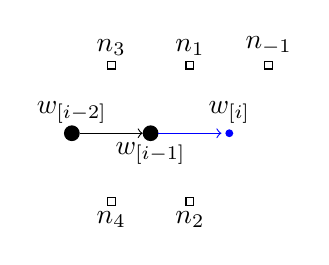
\begin{tikzpicture}
      
      \fill[shift=(180:1)] (0,0) circle [radius=0.1];
      \fill[shift=(180:0)] (0,0) circle [radius=0.1];
      
      \fill[blue](0:1) circle [radius=0.05];
      
      \draw[->] (180:0.9) -- (180:0.1);
      \draw[->, blue] (0:0.1) -- (0:0.9);

	\node[above] at (180:1) {$w_{[i-2]}$};
	\node[below] at (180:0) {$w_{[i-1]}$};
	\node[above] at (0:1) {$w_{[i]}$};

	\foreach \theta in {60,-60,120,-120}{
   	   \draw [shift=(\theta:1)] (-0.05,-0.05) rectangle (0.05,0.05);
  	}
	 \draw [shift=(60:1)] (0.95,-0.05) rectangle (1.05,0.05);
 	\node[above] at (60:1) {$n_1$};
	\node[below] at (-60:1) {$n_2$};
	\node[above] at (120:1) {$n_3$};
	\node[below] at (-120:1) {$n_4$};
	\node[above, shift=(0:1)] at (60:1) {$n_{-1}$};
    \end{tikzpicture}
    \end{minipage}
    
    \begin{minipage}{0.3\hsize}
    \centering
     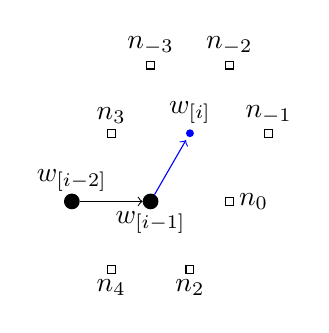
\begin{tikzpicture}
      
      \fill[shift=(180:1)] (0,0) circle [radius=0.1];
      \fill[shift=(180:0)] (0,0) circle [radius=0.1];
      
      \fill[blue](60:1) circle [radius=0.05];
      
      \draw[->] (180:0.9) -- (180:0.1);
      \draw[->, blue] (60:0.1) -- (60:0.9);

	\node[above] at (180:1) {$w_{[i-2]}$};
	\node[below] at (180:0) {$w_{[i-1]}$};
	\node[above] at (60:1) {$w_{[i]}$};


	\foreach \theta in {0,-60,120,-120}{
   	   \draw [shift=(\theta:1)] (-0.05,-0.05) rectangle (0.05,0.05);
  	}
	\draw [shift=(60:1)] (0.95,-0.05) rectangle (1.05,0.05);
	\draw [shift=(60:1), shift=(60:1)] (-0.05,-0.05) rectangle (0.05,0.05);
	\draw [shift=(60:1), shift=(120:1)] (-0.05,-0.05) rectangle (0.05,0.05);
	
 	\node[right] at (0:1) {$n_0$};
	\node[below] at (-60:1) {$n_2$};
	\node[above] at (120:1) {$n_3$};
	\node[below] at (-120:1) {$n_4$};
	\node[above, shift=(0:1)] at (60:1) {$n_{-1}$};
	\node[above, shift=(60:1)] at (60:1) {$n_{-2}$};
	\node[above, shift=(60:1)] at (120:1) {$n_{-3}$};
    \end{tikzpicture}
    \end{minipage}
    
    \begin{minipage}{0.3\hsize}
        \centering
     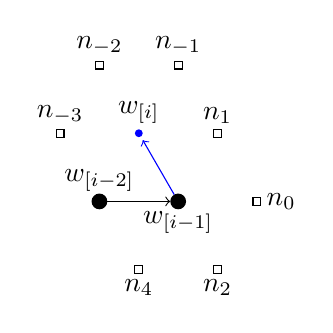
\begin{tikzpicture}
      
      \fill[shift=(180:1)] (0,0) circle [radius=0.1];
      \fill[shift=(180:0)] (0,0) circle [radius=0.1];
      
      \fill[blue](120:1) circle [radius=0.05];
      
      \draw[->] (180:0.9) -- (180:0.1);
      \draw[->, blue] (120:0.1) -- (120:0.9);

	\node[above] at (180:1) {$w_{[i-2]}$};
	\node[below] at (180:0) {$w_{[i-1]}$};
	\node[above] at (120:1) {$w_{[i]}$};


	\foreach \theta in {0,60,-60,-120}{
   	   \draw [shift=(\theta:1)] (-0.05,-0.05) rectangle (0.05,0.05);
  	}
	\draw [shift=(120:1), shift=(60:1)] (-0.05,-0.05) rectangle (0.05,0.05);
	\draw [shift=(120:1), shift=(120:1)] (-0.05,-0.05) rectangle (0.05,0.05);
	\draw [shift=(120:1), shift=(180:1)] (-0.05,-0.05) rectangle (0.05,0.05);
	
 	\node[right] at (0:1) {$n_0$};
	\node[above] at (60:1) {$n_1$};
	\node[below] at (-60:1) {$n_2$};
	\node[below] at (-120:1) {$n_4$};
	\node[above, shift=(120:1)] at (60:1) {$n_{-1}$};
	\node[above, shift=(120:1)] at (120:1) {$n_{-2}$};
	\node[above, shift=(120:1)] at (180:1) {$n_{-3}$};
    \end{tikzpicture}
    \end{minipage}
    \end{tabular}
    \caption{All possible directions of $w[i]$: straight, obtuse, acute.}
    \label{TTT_a3_w}
  \end{center}
\end{figure}

\begin{theorem}[$\delta = 1, \alpha = 4$]
Let $\Xi$ be a unary oritatami system of $\delta = 1, \alpha = 4$. It can yield only finite structures whose size is $O(n^2)$.
\end{theorem}

\begin{lemma}
\label{TTT_a4_2b_lemma}
Any beads which are already stabilized by some bonds use at least two bonds.
\end{lemma}

\begin{proof}[proof of lemma]
Let us consider when $w[i]$ is stabilized by only one bond. See Fig.\ref{TTT_a4_lemma_fig}. According to lemma\ref{TTT_neighbor_lemma}, if $n_3$ is free, $w[i-2]$ has some hands. Thus, $n_4$ has to be occupied in order to stabilize deterministically. Moreover, also $n_2$ has to be occupied for deterministic and also $n_0, n_1$. $n_1$ has some hands because $n_3$ is free. Therefore, $w[i]$ is stabilized at $n_3$ and it has to use at least two hands. It contradict assumption.
\end{proof}

\begin{proof}
According to lemma\ref{TTT_a4_2b_lemma}, when $w[i]$ is stabilized, it has to use at least two bonds. Let us consider when a bead $w[i]$ which is the first bead out of $\hexagon_{w[-n+1]}^n$ is stabilized. See Fig.\ref{TTT_a4_first}. any $n_0, n_1, n_3, n_5$ is free because if some of them is occupied, $w[i]$ is not the first bead out of $\hexagon_{w[-n+1]}^n$. At least two neighbors of $w[i]$ except predecessor have to be occupied in order to bind. In this case, a point which is able to put a bead is only $n_2$. Therefore, any transcript cannot be stabilized in out of $\hexagon_{w[-n+1]}^n$. Hence oritatami system can yield only a finite structure whose size is $O(n^2)$ in $\delta =1, \alpha = 4$.
%lemma???a=4??#bc(C_i) >= #bc(C_{i+1})? ?upper?left
\end{proof}


\begin{figure}
 \centering
    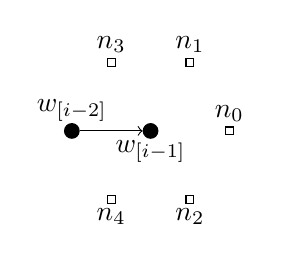
\begin{tikzpicture}
	\fill[shift=(180:1)] (0,0) circle [radius=0.1];
      \fill[shift=(180:0)] (0,0) circle [radius=0.1];
      
      \draw[->] (180:0.9) -- (180:0.1);

	\node[above] at (180:1) {$w_{[i-2]}$};
	\node[below] at (180:0) {$w_{[i-1]}$};
	\node[above] at (0:1) {$n_0$};

	\foreach \theta in {0,60,-60,120,-120}{
   	   \draw [shift=(\theta:1)] (-0.05,-0.05) rectangle (0.05,0.05);
  	}
 	\node[above] at (60:1) {$n_1$};
	\node[below] at (-60:1) {$n_2$};
	\node[above] at (120:1) {$n_3$};
	\node[below] at (-120:1) {$n_4$};
    \end{tikzpicture}
    \caption{$\alpha = 4$: when $w[i]$ is stabilized}
    \label{TTT_a4_lemma_fig}
\end{figure}

\begin{figure}
 \centering
    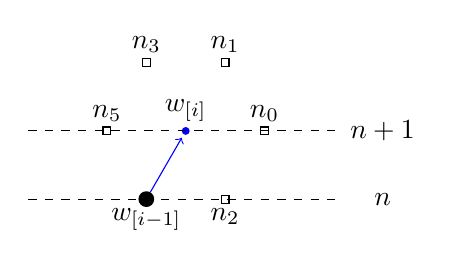
\begin{tikzpicture}
	\fill[shift=(-120:1)] (0,0) circle [radius=0.1];
      \fill[shift=(180:0), blue] (0,0) circle [radius=0.05];
      
      \draw[dashed] (180:2) -- (0:2);
      \draw[dashed, shift=(-60:1)] (180:2.5) -- (0:1.5);
      \draw[->, blue] (-120:0.9) -- (-120:0.1);

	\node[below] at (-120:1) {$w_{[i-1]}$};
	\node[above] at (180:0) {$w_{[i]}$};
	\node[above] at (0:1) {$n_0$};

	\foreach \theta in {0,60,-60,120,180}{
   	   \draw [shift=(\theta:1)] (-0.05,-0.05) rectangle (0.05,0.05);
  	}

 	\node[above] at (60:1) {$n_1$};
	\node[below] at (-60:1) {$n_2$};
	\node[above] at (120:1) {$n_3$};
	\node[above] at (180:1) {$n_5$};
	
	\node at (0:2.5) {$n+1$};
	\node[shift=(-60:1)] at (0:2) {$n$};
    \end{tikzpicture}
    \caption{the first bead out of $\hexagon_{w[-n+1]}^n$}
    \label{TTT_a4_first}
\end{figure}

